\documentclass[12pt]{article}

\usepackage[T2A]{fontenc}
\usepackage[utf8]{inputenc}
\usepackage[russian]{babel}

\usepackage{mathtext}
\usepackage{cmap}
\usepackage{amsmath,amssymb,amsthm,amscd,amsfonts}
\usepackage{graphicx}
\usepackage[colorbox,usenames,dvipsnames]{xcolor}
\usepackage{float, caption, subcaption, multirow}
\usepackage[section]{minted}
\usepackage{hyperref}

\voffset -24.5mm
\hoffset -5mm
\textwidth 173mm
\textheight 240mm
\oddsidemargin=0mm \evensidemargin=0mm

\definecolor{codegray}{gray}{0.9}
\newcommand{\code}[1]{\colorbox{codegray}{\texttt{#1}}}
\newmintinline[src]{console}{}

\renewcommand{\theFancyVerbLine}{\sffamily\textcolor{black}{\scriptsize\oldstylenums{\arabic{FancyVerbLine}}}}
\usemintedstyle[console]{bw}
\setminted[console] {
     bgcolor = white,
     linenos = false,
     tabsize = 2,
     formatcom = \color{black},
     frame = leftline,
     framerule = 0.8pt,
     framesep = 0.5cm,
     xleftmargin = 1cm,
     xbottommargin = 0.1cm
     breaklines = true,
     escapeinside=<>
}
\usemintedstyle[ruby]{tango}
\setminted[ruby] {
     bgcolor = white,
     linenos = true,
     tabsize = 2,
     formatcom = \color{black},
     frame = leftline,
     framerule = 0.8pt,
     framesep = 0.5cm,
     xleftmargin = 1cm,
     xbottommargin = 0.1cm
     breaklines = true,
     escapeinside=||
}

\hypersetup{linkcolor=blue, urlcolor=blue, colorlinks=true}

\begin{document}

\title{
    Лабораторная работа №5 \\ 
    Дисциплина <<Методы и средства защиты информации>> \\ 
    Metasploit}
\author{Евгений Хандыго, гр. 53501/3}

\maketitle
\tableofcontents

\newpage

\section{Постановка задачи}

В рамках данной работы необходимо овладеть основными аспектами работы с утилитой gpg4win. Ход работы соответствует следующим пунктам:
\begin{itemize}
    \item Изучить документацию gpg и gpg4win.
    \item Поставить собственную ЭЦП на файл.
    \item Проверить ЭЦП на стороннем файле.
    \item Обменяться зашифрованными сообщениями с другим пользователем gpg.
    \item Потренироваться в использовании утилиты gpg через интерфейс командной строки.
\end{itemize}
\section{Система оценивания SSL Server Test} \label{sct:best-practices}

В данном разделе будет приведена система ранжирования доменов, а также представлены развернутые расшифровки для некоторых других полей
отчета, генерируемого SSL Server Test.

\subsection{Сводка}

В данном разделе представлены:
\begin{itemize}
    \item Общая оценка анализируемого домена по шестибальной шкале.
    \item Оценка сертификата анализируемого домена по стобальной шкале \footnote{на самом деле, похоже, возможны только оценки $0$ и 
        $100$}.
    \item Оценка протоколов, поддерживаемых на анализируемом домене, по стобальной шкале. 
    \item Оценка алгоритмов обмена ключами (на стадии создания сессии), поддерживаемых на анализируемом домене, по 
        стобальной шкале.
    \item Оценка мощности алгоритмов симметричного шифрования, поддерживаемых на анализируемом домене, по стобальной шкале. 
\end{itemize}
Общая оценка для домена формируется путем аггрегации оценок для трех последних из представленных категорий и квантования результата. 

Домен получает оценку $100$ в графе <<сертификат>> в случае, если его сертификат отвечает всем <<разумным>> требованиям безопасности 
таким, например, как:
\begin{itemize}
    \item Доменное имя совпадает с указанным в сертификате. 
    \item Сертификат действителен.
    \item Срок действия сертификата не истек.
    \item Подлинность сертификата подтверждается сторонней сущностью (сертификат не является самоподписанным).
    \item Сертификат не отозван.
\end{itemize}
Также стоит отметить, что некоторые организации создают и распространяют собственные приватные CA-сертификаты. Использование 
приватных CA может привести к тому, что сервис SSL Server Test будет не в состоянии подтвердить подлинность и достоверность 
сертификата на анализируемом домене (без доступа к приватным сертиыикатам CA). Оценки во всех остальных категориях строятся путем
аггрегации константных весовых коэффициентов, присваиваемых возможным в рамках данных категорий опциям. 

\subsection{Конфигурация} \label{ssct:best-practices.configuration}

В данном разделе представлены поддерживаемые на анализируемом сервере шифры, при этом используется следующая нотация: каждый шифр
представляется в форме \\ \code{P\_KEAAA\_WITH\_MEA\_HA}, где 
\begin{itemize}
    \item \code{P} (protocol) --- протокол.
    \item \code{KEAAA} (key exchange and authentication algorithms) --- алгоритмы обмена ключами и аутентификации. Данный токен 
        может представлять единственный алгоритм (в этом случае этот алгоритм используется на обеих стадиях) или в виде 
        \code{KEA\_AA}, где \code{KEA} (key exchange algorithm) и \code{AA} (authentication algorithm) представляют алгоритмы, 
        используемые на стадиях создания сессии и аутентификации, соответственно.
    \item \code{WITH} --- ключевое слово-разделитель.
    \item \code{MEA} (message encryption algorithm) --- симметричный алгоритм шифрования сообщений.
    \item \code{HA} (hashing algorithm) --- алгоритм хэширования, используемый для обеспечения целостности пакетов в SSL/TLS.
\end{itemize}
В дальнейшем мы будем ссылаться на данное представление, приводя расшифровки только для конкретных алгоритмов.

\subsection{Детали протокола} \label{ssct:best-practices.protocol-details}

В данном разделе собрана различная информация о реализации протокла на анализируемом домене такая как, например, подверженность 
известным атакам и поддержка опций.

\subsubsection{DROWN}

\textbf{DROWN} --- это относительно новая (март $2016$ года) уязвимость, ставящая под угрозу 
\href{https://drownattack.com/top-sites.html}{множество ресурсов} в публичной сети, использующих HTTPS (в том числе и TLS). 
Уязвимость данного типа является особенно опасной, поскольку ее эксплуатация возможна даже для серверов, которые сконфигурированы в 
соответствии с лучшими рекомендациями. В общем случае уязвимость типа DROWN может эксплуатироваться в трех случаях:
\begin{itemize}
    \item Сервер поддерживает SSLv2. 
    \item Сервер, поддерживающий SSLv2 может быть использован для атаки любых других серверов, использующих такой же RSA-ключ.
    \item Сервер, поддерживающий SSLv2, а также использующий \href{https://www.openssl.org/news/secadv/20160301.txt}{уязвимые 
        версии OpenSSL}, может быть использован для атаки любых доменов, указанных в его сертификате.
\end{itemize}
Таким образом, уязвимость домена атаке типа DROWN не может быть подтверждена или опровергнута путем анализа конфигурации только лишь 
целевого домена: необходимо также проверить использование RSA-ключей и упоминание имени рассматриваемого домена где-либо еще. Для 
осуществление такого рода проверки SSL Server Test использует поисковую систему \href{https://censys.io/}{Censys} в сочетании с 
собственными алгоритмами проверки в режиме реального времени. Подверженность атаке этого типа приводит к снижению общей оценки 
юезопасности домена до \code{F}. 

\subsubsection{Безопасное переподключение}

Под \textbf{переподключением} (renegotiation) здесь понимается способность сервера открывать новое безопасное соединение, используя 
одно из уже существующих. Такая опция полезна в случае реализации некоторых сценариев таких, например, как авторизация пользователя 
сайта, который уже проделал какие-то действия анонимно и результат этих действий необходимо сохранить. Первые реализации опции 
переподключения в SSLv3 и TLS не обеспечивали достаточно сильного <<связывания>> запроса на переподключение с текущей активной 
сессией, что позволяло провести атаку типа <<посредник>>, при которой злоумышленник мог получить право к проведению экслюзивных 
пользовательских операций. В последующих версиях, конечно, данная уязвимость была исправлена. Исправленная (пропатченная) реализация
переподключения получила название \textbf{безопасного переподключения} (secure renegotiation).

\subsubsection{BEAST} \label{sssct:BEAST}

Протоколы семейства SSL до версии TLS $1.0$ обладают серьезным недостатком: инициализирующий вектор (initialization vector, IV),
использующийся для стохастизации шифр-текста в режиме сцепления блоко (cipher block chaining, CBC), может быть предсказан посредством
атаки типа <<активный посредник>>. Предсказание значения инициализирующего вектора делает возможным расшифровку небольших пакетов
данных, пересылаемых от клиента к серверу, в случае, если злоумышленник может предположить, что зашифровано в данном пакете. Может
показаться, что атака такого рода не несет существенной опасности, поскольку для расшифровки одного конкретного пакета необходимо
сделать достаточно большое количество предположений о его содержимом. Однако существуют пакеты, инкапсулирующие крайне важную 
информацию, 
размер которых достаточно мал, а содержимое может быть частично известно злоумышленнику. К числу таких пакетов можно отнести 
сессионные куки (cookies) в HTTP и аутентификационные данные. 
Для того, чтобы избежать атаки типа <<BEAST>> со стороны сервера можно
прибегнуть к следующим мерам:
\begin{itemize}
    \item Отключить поддержку протоколов семейства SSL до TLS $1.0$ включительно. 
    \item Включить режим приоритеризации шифров и выбрать в качестве наиболее желаемого шифра RC4 (RC4 является потоковым шифром и
        потому не имеет инициализирующего вектора).
\end{itemize}
Ни одна из этих мер не является <<серебрянной пулей>> поскольку:
\begin{itemize}
    \item Возможно, не все клиенты готовы поддерживать TLS $1.1+$.
    \item Существуют атаки, направленные на понижение версии (downgrade) используемого протокола так, что уязвимости старых версий
        снова могут быть использованы.
    \item \href{http://blog.cryptographyengineering.com/2013/03/attack-of-week-rc4-is-kind-of-broken-in.html}{RC4 взломан}.  
\end{itemize}
Таким образом, необходимо использовать более продвинутые версии алгоритмов шифрования или... 
На самом деле BEAST --- это исключительно клиентская уязвимость. На стороне клиента избежать атак данного вида можно с помощью 
техники \href{https://bugzilla.mozilla.org/show_bug.cgi?id=665814#c59}{разделения $1 / n - 1$} ($1 / n - 1$ split). 
В разделе 
<<Детали протокола>> SSL Server Test включает информацию о том, предприняты ли меры относительно BEAST со стороны сервера. Никаких 
оценочных штрафов по причине того, что большиснвто браузеров давно используют метод разделения $1 / n - 1$, не предусмотрено.

\subsubsection{POODLE}

POODLE стал последней каплей для SSL (не TLS). В октябре $2014$го было обнаружено, что SSLv3 (и все предыдущие версии, конечно)
подвержены новому типу атаки --- POODLE. Позже, в декабре того же года, выяснилось, что некоторые реализации TLS также позволяют 
эксплуатировать эту уязвимость. Корень проблемы лежит в самых основах SSL, а именно в том, что аутентификация данных производится
до их шифровки. Это значит, что получатель сообщения должен сделать некоторую криптографическую операцию до того, как 
аутентифицировать сообщение. Чаще всего это приводит к краху (DOOM principle) всего протокола, что и произошло с SSL. На этапе,
когда уязвимым считался только SSL, решение лежало на поверхности: отказаться от поддержки SSLv3 на сервере (для того, чтобы 
атакующий не смог понизить версию до нее и исользовать уязвимость). С TLS все тоже оказалось достаточно легко --- достаточно 
применить патч. 

\subsubsection{Предотвращение нежелательного понижения версии протокола}

Как уже обсуждалось выше, понижение версии протокола (version downgrade) во многих случаях крайне нежелательно, поскольку позволяет 
злоумышленнику эксплуатировать уязвимости протоколов старых версий (если сервер их поддерживает). Для того, чтобы предотвратить 
атаки этого типа в спецификацию TLS был добавлен особенный особенный токен шифра \code{TLS\_FALLBACK\_SCSV} (
\href{https://datatracker.ietf.org/doc/rfc7507/?include_text=1}{RFC $7507$}), который не соответствует никакому шифру, но задает
определенное поведение для клиента и сервера в случае, если такой токен включен в список шифров, поддерживаемых клиентом. 
Определяемое поведение по факту запрещает использовать версию протокола ниже максимальной поддерживаемой на сервере. 

\subsubsection{CRIME}

CRIME, наверное, нельзя назвать атакой. Однако, эксплуатация этой <<уязвимости>> помогает злоумышленнику получить больше знаний о
виде открытого текста. В основе CRIME лежит следующая идея: внутрь пакетов, посылаемых на сервер встраивается дополнительный 
контент. При этом, если включено сжатие данных и злоумышленник способен измерять размер переланных сообщений, то при понижении 
размера сжатого сообщения можно сделать вывод о том, что дополнительный встроенный текст и оригинальный открытый текст содержат
некоторое количество одинаковых символов. Конечно, для эксплуатации данной уязвимости, злоумышленнику необходимо внедрить 
дополнительную логику на стороне клиента, поэтому проблема может считаться исключительно клиентской. Таким образом, защита от 
CRIME достигается путем отключения опции сжатия данных на стороне клиента и/или сервера. 

\subsubsection{Heartbleed}

Heartbleed --- уязвимость, появившаяся не из дизайна самого протокола, но из-за ошибки реализации. Эксплуатация данной уязвимости
возможна только для некоторых версий OpenSSL поверх расширения проверки пульса (heartbeat extension) для TLS. Ошибка в программе 
позволяла получить некоторые скрытые в обычном случае данные с сервера, в том числе и его приватный ключ. Позже был выпущен патч,
устраняющий данную проблему. Конечно, для того, чтобы убедиться, что трафик от сервера не скомпрометирован, после установки
патча необходимо установить новый сертификат и отменить действие старого. Несмотря на то, что данная уязвимость была обнаружена
около двух лет назад, SSL Server Test все еще осуществляет ее проверку. В свете этой проблемы использование так называемого 
расширения продолжительной защищенности (forward secrecy, см. ниже) стало особенно важно.

\subsubsection{OpenSSL CCS. CVE-2014-0224}

Данная уязвимость также специфична только для OpenSSL и существовала в коде более пятнадцати лет. Эксплуатация данной уязвимости 
позволяет злоумышленнику указать пустой мастер-ключ, использующийся затем для генерации сессионного ключа.

\subsubsection{OpenSSL Padding Oracle. CVE-2016-2107} \label{sssct:OpenSSLPO}

Относительно новая уязвимость, обнаруженная в марте этого года в последних версиях OpenSSL. Подобно POODLE, в процессе эксплуатации
данной уязвимости последовательно модифицируются биты шифр-текста. Как и в случае POODLE, проблема лежит в неправильном порядке 
операций аутентификации и шифровки, что снова подтверждает достоверность принципа краха (DOOM principle). 

\subsubsection{Продолжительная защищенность}

\emph{Продолжительная защищенность} (\emph{forward secrecy}) --- это свойство некоторых шифров, заключающаеся в том, что для взлома 
записанной истории шифрованных сообщений недостаточно получить только лишь приватный ключ сервера. Например, при использовании RSA 
симметричный ключ шифра генерируется на стороне сервера и затем посылается клиенту. Конечно, ключ посылается в виде шифр-текста, 
защищенного приватным ключом сервера. В случае, если злоумышленник может записывать весь трафик, идущий с сервера, то при получении
в будущем приватного ключа единственного хоста, у него появится возможность взломать весь записанный до этого трафик. В противовес,
например, при использовании алгоритма Диффи-Хеллмана на этапе создания сессии, ключ шифруется ассимметричным способом, что делает
описанный выше вариант событий невозможным. 

\subsubsection{Другие категории}

Ниже представлен список некоторых других опций, отображаемых в разделе <<Конфигурация протокола>> SSL Server Test. 
\begin{itemize}
    \item \textbf{NPN} (\emph{Next Protocol Negotiation}). С появлением новых сетевых протоколов уровня приложений, в особенности
        HTTP/2, появилась необходимость предоставить возможность выбора, какой из протоколов этого уровня использовать. NPN --- 
        первая попытка расширения TLS в этом направлении. Для обеспечения необходимой функциональности в процесс рукопожатия была 
        добавлен еще один этап: в первый ответ сервера включалась информация о поддерживаемых им протоколах уровня приложений, после
        чего клиент должен был ответить выбором из представленных опций.
    \item \textbf{ALPN} (\emph{Application-Layer Protocol Negotiation Extension},  \href{https://tools.ietf.org/html/rfc7301}{RFC 
        7301}). Данное расширение TLS является улучшением NPN. Его отличие от предшественника заключается в том, что список 
        протоколов, поддерживаемых на уровне приложений, формируется клиентом и включается им в первый запрос к серверу на стадии
        рукопожатия. Такой подход позволяет сократить количество сообщений, которыми обмениваются клиент и сервер на стадии 
        рукопожатия. 
    \item \textbf{Возобновление сессии} (session resumption, \href{https://tools.ietf.org/html/rfc5077}{RFC 5077}). Данное 
        расширение позволяет клиенту возобновить защищенное соединение с сервером через некоторое (определенное) время после его 
        закрытия. Существует две реализации данной функциональности: кэширование сессионых ключей на стороне сервера и выдача 
        сервером билетов (tickets). Первый подход является необоснованно дорогим в случае, когда сервер должен поддерживать большое 
        количество параллельных соединений: необходимо периодически сгружать данные на диск (что уже само по себе не является 
        кэшированием), поддерживать их согласованность (в случае распределенных систем, например) и сохранность. По причине этих 
        сложностей от подхода с кэшированием быстро отказались в силу билетов. Под билетом в данном случае подразумевается некоторая
        сущность, которая создается сервером, шифруется только ему известным ключом и им же обрабатывается для восстановления 
        сессии. Билеты хранятся на стороне клиента, что существенно снижает нагрузку на сервер по сравнению с кэширующим подходом.
    \item \textbf{OCSP сшивание} (Online Certificate State Protocol (OCSP) stapling). Для проверки аннулированности сертификата 
        изначально был предложен так называемый протокол состояния сертификата (OSCP). Суть его заключается в том, что ключевые
        CA предоставляют сервис для проверки аннулированности сертификатов, подписанных ими. Главный недостаток такого подхода 
        заключается в том, такие сервисы должны выдерживать очень большую нагрузку (например, в случае одновременного подключения
        тысяч клиентов к некоторому домену). Для того, чтобы нивелировать этот недостаток был предложен следующий подход: приветствие
        от сервера  включает в себя (подшитый) ответ о статусе сертификата уелевого сервера, подписанный ответственным CA и, 
        содержащий метку времени. Подпись CA в данном случае обеспечивает безопасность данных, а метка времени времени позволяет
        судить ою актуальности предоставленной ннформации. В случае, если приветствие от сервера не будет содержать необходимой 
        информации, клиент все еще имеет возможность обратиться к CA напрямую, используя OCSP.
    \item \textbf{Строгая безопасность транспортного уровня} ((HTTP) Strict Transport Security (HSTS), 
        \href{https://tools.ietf.org/html/rfc6797}{RFC 6797}). Данный механизм был разработан для того, чтобы обеспечить 
        принудительную защищенность сетевого протокола транспортного уровня. В случае включения этой опции на сервере, при 
        обращении к нему по HTTP, в приветсвии к клиенту будет указан особый заголовок. Согласно спецификации клиент должен 
        отреагировать на этот заголовок следующим образом: на протяжении указанного в заголовке времени, все запросы, адрессованные
        данному домену и все ссылки на него должны быть принудительно переписаны таким образом, чтобы начинаться с \code{https}.
        Такой подход делает невозможным атаки, направленные на понижение протокола (от HTTPS к HTTP), хотя, конечно, не обеспечивает
        безопасности при первом подключении к ресурсу, но только по HTTP.
    \item \textbf{Зпоминание публичных HTTP ключей} (HTTP Public Key Pinning, \href{https://tools.ietf.org/html/rfc7469}{RFC 7469}).
        Данный механизм вводит особое понятие булавки (pin), которая описывает связь между доменом и цепью его сертификатов. 
        Согласно спецификации данное расширение обязывает клиента запоминать цепь сертификатов для домена и сверять ее при всяком
        повторном доступе. Такой подход позволяет на ранней стадии определить небезопасность домена в случае, например, если его CA 
        был скомпрометирован.
    \item \textbf{Отказ в длинном рукопожатии} (long handshake intolerance). Данное поведение присуще к некоторым реализациям 
        TLS, которые не способны обрабатывать приветствие длинной более $255$ти символов, хотя в спецификации протокола не 
        накладывается никаких ограничений на размер приветственного сообщения.  
    \item \textbf{Отказ от версии} (version intolerance). На этапе рукопожатия первом делом сервер и клиент должны достичь согласия 
        о версии используемого протокола: клиент сообщает максимальную версию протокола, которую поддерживает, в ответ сервер 
        высылает максимально доступную версию из предоставленных клиентом и известных ему самому. В общем случае сервер не должен
        полагаться на какую-либо стороннюю информацию о протоколе и должен принять решение, исходя только лишь из номера версии. 
        Таким образом, клиент может указать любой номер версии, даже несуществующий. Сервер в этом случае тем не менее должен 
        отработать корректно. К сожалению, существуют реализации TLS, которые не поддерживают такого поведения и могут отказать
        клиенту в соединении, если указана несуществующая версия (при этом поведение может варьироваться, в зависимости от 
        минорного/мажорного номера версии). Такое поведение и принято называть отказом от версии.
\end{itemize}
\section{Лучший за последнее время}

В разделе <<Лучшие за последнее время>> был выбран домен foxbox.pw. 

\begin{figure}[H]
    \centering
    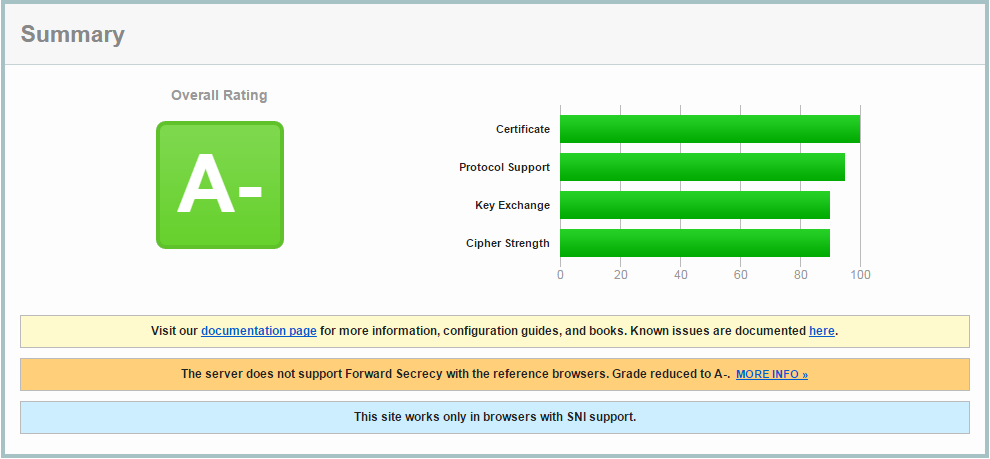
\includegraphics[width=\textwidth]{resources/01_summary.png}
    \caption{Сводка по домену foxbox.pw}
    \label{fig:01-summary}
\end{figure}

Оценка домена была снижена с \code{A} до \code{A-} поскольку продолжительная защищенность поддерживается не со всеми эталонными 
клиентами (браузерами).

Ниже приведена таблица рассшифровок шифров, доступных для использования на рассматриваемом домене. Колонки таблицы зашифрованы 
согласно нотации, представленной в разделе \ref{ssct:best-practices.configuration}.

\begin{table}[H]
    \centering
    \begin{tabular}{c|c|c|c|c|c}
        \textbf{P} & \textbf{KEA} & \textbf{AA} & \textbf{MEA} & \textbf{Мощность} & \textbf{HA} \\ 
        \hline
        TLS & RSA & RSA & 3DES\_EDE\_CBC & $168$ & SHA \\
        TLS & ECDHE & RSA & 3DES\_EDE\_CBC & $168$ & SHA \\
        TLS & RSA & RSA & AES\_128\_CBC & $128$ & SHA \\
        TLS & RSA & RSA & CAMELLIA\_128\_CBC & $128$ & SHA \\
        TLS & ECDHE & RSA & AES\_128\_CBC & $128$ & SHA \\
        TLS & RSA & RSA & AES\_128\_CBC & $128$ & SHA256 \\
        TLS & RSA & RSA & AES\_128\_GCM & $128$ & SHA256 \\
        TLS & ECDHE & RSA & AES\_128\_CBC & $128$ & SHA256 \\
        TLS & ECDHE & RSA & AES\_128\_GCM & $128$ & SHA256 \\
        TLS & RSA & RSA & AES\_256\_CBC & $256$ & SHA \\
        TLS & RSA & RSA & CAMELLIA\_256\_CBC & $256$ & SHA \\
        TLS & ECDHE & RSA & AES\_256\_CBC & $256$ & SHA \\
        TLS & RSA & RSA & AES\_256\_CBC & $256$ & SHA256 \\
        TLS & RSA & RSA & AES\_256\_GCM & $256$ & SHA256 \\
        TLS & RSA & RSA & AES\_256\_GCM & $256$ & SHA384 \\
        TLS & ECDHE & RSA & AES\_256\_CBC & $256$ & SHA384 \\
        TLS & ECDHE & RSA & AES\_256\_GCM & $256$ & SHA384 \\
    \end{tabular}
    \caption{Шифры, доступные на foxbox.pw}
    \label{tbl:01-cipher-suits}
\end{table}

Приведем теперь разбор некоторых деталий реализации протокола на рассматриваемом домене по категориям, рассмотренным в секции 
\ref{ssct:best-practices.protocol-details}

\begin{table}[H]
    \centering
    \begin{tabular}{c|c}
        \hline
        \multicolumn{2}{c}{\textbf{Уязвимости}} \\ \hline
        \textbf{Уязвимость} & \textbf{Уязвим} \\ \hline
        \textbf{DROWN} & Нет \\
        \textbf{BEAST} & Да, со стороны сервера \\
        \textbf{POODLE} & Нет \\
        \textbf{Атака на понижение версии} & Нет \\
        \textbf{Heartbleed} & Нет \\
        \textbf{OpenSSL CCS} & Нет \\
        \textbf{OpenSSL Padding Oracle} & Нет \\ \hline
        \multicolumn{2}{c}{\textbf{Опции}} \\ \hline
        \textbf{Опция} & \textbf{Включена} \\ \hline 
        \textbf{Безопасное переподключение} & Да \\ 
        \textbf{Сжатие данных} & Нет \\ 
        \textbf{Пульс} & Да \\ 
        \textbf{Продожительная защищенность} & Нет \\ 
        \textbf{ALPN} & Нет \\ 
        \textbf{NPN} & Да (HTTP/1.1) \\ 
        \textbf{Возобновление сессии (кэширование)} & Нет \\
        \textbf{Возобновление сессии (билеты)} & Да  \\
        \textbf{OCSP сшивание} & Да  \\
        \textbf{HSTS} & Нет \\ 
        \textbf{HPKP} & Нет \\ 
        \textbf{Отказ в длинном рукопожатии} & Нет \\ 
        \textbf{Отказ от версии} & Нет \\ 
    \end{tabular}
    \caption{Детали реализации протокола на foxbox.pw}
    \label{01-protocol-details}
\end{table}

Рассматриваемый домен поддерживает только протокол TLS, что уже свидетельствует о его не самой плохой защищенности. Кроме того, 
как видно из таблицы \ref{tbl:01-cipher-suits}, рассматриваемый домен не поддерживает RSA в качестве шифра для сообщений, что также
является большим плюсом. К тому же домен не подвержен ни одной известной SSL Server Test уязвимости (BEAST не считается --- полностью
клиентская уязвимость, как показано в разделе \ref{sssct:BEAST}). Единственным недостатком является частично не поддерживаемая 
продолжительная защищенность. 
\section{Худший за последнее время}

В разделе <<Худшие за последнее время>> был выбран домен tyranoff.ru. 

\begin{figure}[H]
    \centering
    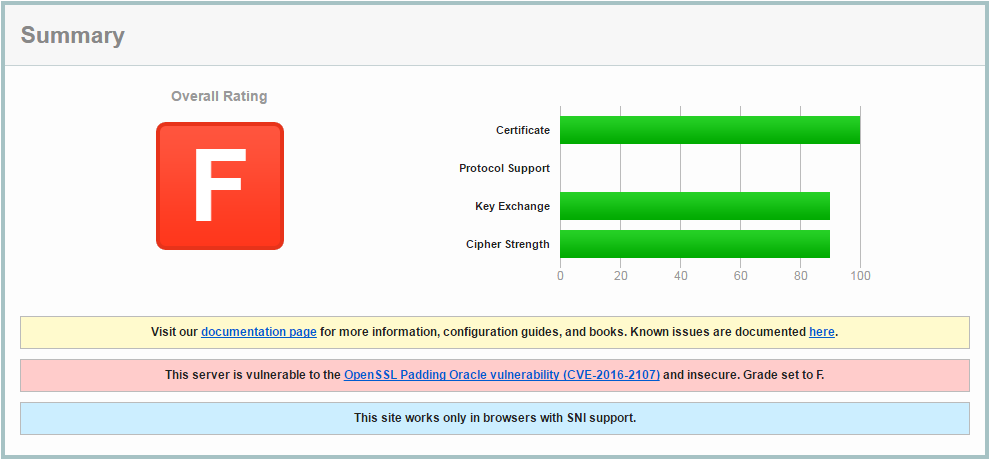
\includegraphics[width=\textwidth]{resources/02_summary.png}
    \caption{Сводка по домену tyranoff.ru}
    \label{fig:02-summary}
\end{figure}

Оценка домена была снижена до \code{F} поскольку обнаружена уязвимость к атаке OpenSSL Padding Oracle.

Ниже приведена таблица рассшифровок шифров, доступных для использования на рассматриваемом домене. Колонки таблицы зашифрованы 
согласно нотации, представленной в разделе \ref{ssct:best-practices.configuration}.

\begin{table}[H]
    \centering
    \begin{tabular}{c|c|c|c|c|c}
        \textbf{P} & \textbf{KEA} & \textbf{AA} & \textbf{MEA} & \textbf{Мощность} & \textbf{HA} \\ 
        \hline
        TLS & ECDHE & RSA & AES\_128\_GCM & $128$ & SHA256 \\
        TLS & ECDHE & RSA & AES\_128\_CBC & $128$ & SHA256 \\
        TLS & ECDHE & RSA & AES\_128\_CBC & $128$ & SHA \\
        TLS & ECDHE & RSA & AES\_256\_GCM & $256$ & SHA384 \\
        TLS & ECDHE & RSA & AES\_256\_CBC & $256$ & SHA384 \\
        TLS & ECDHE & RSA & AES\_256\_CBC & $256$ & SHA \\
        TLS & DHE & RSA & AES\_256\_GCM & $256$ & SHA384 \\
        TLS & DHE & RSA & AES\_256\_CBC & $256$ & SHA256 \\
        TLS & DHE & RSA & AES\_256\_CBC & $256$ & SHA \\
        TLS & DHE & RSA & AES\_128\_GCM & $128$ & SHA256 \\
        TLS & DHE & RSA & AES\_128\_CBC & $128$ & SHA256 \\
        TLS & DHE & RSA & AES\_128\_CBC & $128$ & SHA \\
        TLS & RSA & RSA & AES\_256\_CBC & $128$ & SHA \\
        TLS & RSA & RSA & AES\_128\_GCM & $128$ & SHA256 \\
        TLS & RSA & RSA & AES\_128\_CBC & $128$ & SHA256 \\
        TLS & DHE & RSA & 3DES\_EDE\_CBC & $112$ & SHA \\
        TLS & RSA & RSA & 3DES\_EDE\_CBC & $112$ & SHA \\
    \end{tabular}
    \caption{Шифры, доступные на tyranoff.ru}
    \label{tbl:02-cipher-suits}
\end{table}

Приведем теперь разбор некоторых деталий реализации протокола на рассматриваемом домене по категориям, рассмотренным в секции 
\ref{ssct:best-practices.protocol-details}

\begin{table}[H]
    \centering
    \begin{tabular}{c|c}
        \hline
        \multicolumn{2}{c}{\textbf{Уязвимости}} \\ \hline
        \textbf{Уязвимость} & \textbf{Уязвим} \\ \hline
        \textbf{DROWN} & Нет \\
        \textbf{BEAST} & Да, со стороны сервера \\
        \textbf{POODLE} & Нет \\
        \textbf{Атака на понижение версии} & Нет \\
        \textbf{Heartbleed} & Нет \\
        \textbf{OpenSSL CCS} & Нет \\
        \textbf{OpenSSL Padding Oracle} & Да \\ \hline
        \multicolumn{2}{c}{\textbf{Опции}} \\ \hline
        \textbf{Опция} & \textbf{Включена} \\ \hline 
        \textbf{Безопасное переподключение} & Да \\ 
        \textbf{Сжатие данных} & Нет \\ 
        \textbf{Пульс} & Да \\ 
        \textbf{Продожительная защищенность} & Да \\ 
        \textbf{ALPN} & Да \\ 
        \textbf{NPN} & Да (HTTP/1.1) \\ 
        \textbf{Возобновление сессии (кэширование)} & Да \\
        \textbf{Возобновление сессии (билеты)} & Да  \\
        \textbf{OCSP сшивание} & Нет  \\
        \textbf{HSTS} & Нет \\ 
        \textbf{HPKP} & Нет \\ 
        \textbf{Отказ в длинном рукопожатии} & Нет \\ 
        \textbf{Отказ от версии} & Нет \\ 
    \end{tabular}
    \caption{Детали реализации протокола на tyranoff.ru}
    \label{01-protocol-details}
\end{table}

Рассматриваемый домен использует тольк оверсии протокола TLS, однако уязвим к OpenSSL Padding Oracle (см. \ref{sssct:OpenSSLPO}).
В остальном настройка домена выглядит достаточно неплохо, включая почти полную поддержку продолжительной защищенности. Некоторое 
недоумение вызывают только одновременное использование таких опций, как ALPN/NPN и возобновление сессии через кэширование/билеты.
Конфигурацию сервера можно улучшить следующим образом:
\begin{itemize}
    \item Отключить поддержку ALPN, если не предполагается использование HTTP/2.
    \item Отключить кэширование сессий. 
    \item Пропатчить версию OpenSSL, обновить сертификат.
    \item Включить такие опции, как <<OSCP сшивание>> и HSTS. 
\end{itemize}
\section{Произволный домен}

В качестве произвольного домена для анализа был выбран ru.sharelatex.com. 

\begin{figure}[H]
    \centering
    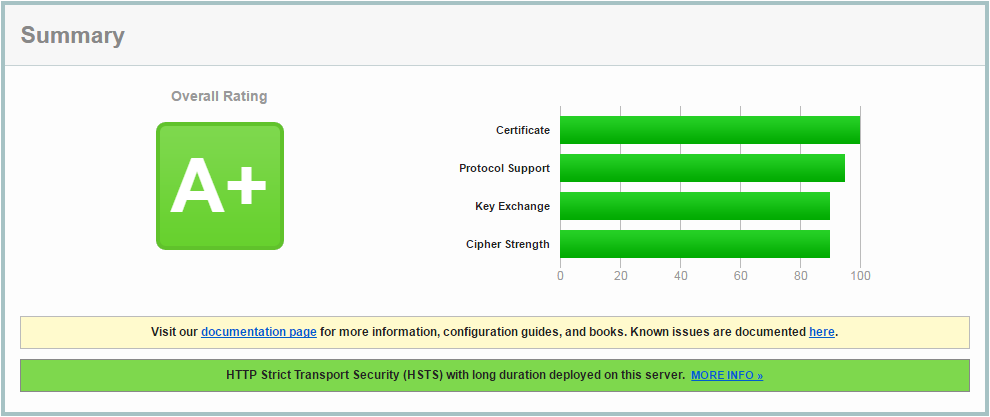
\includegraphics[width=\textwidth]{resources/03_summary.png}
    \caption{Сводка по домену ru.sharelatex.com}
    \label{fig:03-summary}
\end{figure}

Оценка домена была улучшена до \code{A+} поскольку включена поддержка HSTS с достаточно длинным периодом времени.

Ниже приведена таблица рассшифровок шифров, доступных для использования на рассматриваемом домене. Колонки таблицы зашифрованы 
согласно нотации, представленной в разделе \ref{ssct:best-practices.configuration}.

\begin{table}[H]
    \centering
    \begin{tabular}{c|c|c|c|c|c}
        \textbf{P} & \textbf{KEA} & \textbf{AA} & \textbf{MEA} & \textbf{Мощность} & \textbf{HA} \\ 
        \hline
        TLS & ECDHE & RSA & AES\_128\_GCM & $128$ & SHA256 \\
        TLS & ECDHE & RSA & AES\_128\_CBC & $128$ & SHA256 \\
        TLS & ECDHE & RSA & AES\_128\_CBC & $128$ & SHA \\
        TLS & RSA & RSA & AES\_128\_GCM & $128$ & SHA256 \\
        TLS & RSA & RSA & AES\_128\_CBC & $128$ & SHA256 \\
        TLS & RSA & RSA & AES\_128\_CBC & $128$ & SHA \\
        TLS & ECDHE & RSA & AES\_256\_GCM & $256$ & SHA384 \\
        TLS & ECDHE & RSA & AES\_256\_CBC & $256$ & SHA384 \\
        TLS & ECDHE & RSA & AES\_256\_CBC & $256$ & SHA \\
        TLS & RSA & RSA & AES\_256\_GCM & $256$ & SHA384 \\
        TLS & RSA & RSA & AES\_256\_CBC & $256$ & SHA256 \\
        TLS & RSA & RSA & AES\_256\_CBC & $256$ & SHA \\
        TLS & ECDHE & RSA & 3DES\_EDE\_CBC & $112$ & SHA \\
        TLS & RSA & RSA & 3DES\_EDE\_CBC & $112$ & SHA \\
    \end{tabular}
    \caption{Шифры, доступные на ru.sharelatex.com}
    \label{tbl:03-cipher-suits}
\end{table}

Приведем теперь разбор некоторых деталий реализации протокола на рассматриваемом домене по категориям, рассмотренным в секции 
\ref{ssct:best-practices.protocol-details}

\begin{table}[H]
    \centering
    \begin{tabular}{c|c}
        \hline
        \multicolumn{2}{c}{\textbf{Уязвимости}} \\ \hline
        \textbf{Уязвимость} & \textbf{Уязвим} \\ \hline
        \textbf{DROWN} & Нет \\
        \textbf{BEAST} & Да, со стороны сервера \\
        \textbf{POODLE} & Нет \\
        \textbf{Атака на понижение версии} & Нет \\
        \textbf{Heartbleed} & Нет \\
        \textbf{OpenSSL CCS} & Нет \\
        \textbf{OpenSSL Padding Oracle} & Нет \\ \hline
        \multicolumn{2}{c}{\textbf{Опции}} \\ \hline
        \textbf{Опция} & \textbf{Включена} \\ \hline 
        \textbf{Безопасное переподключение} & Да \\ 
        \textbf{Сжатие данных} & Нет \\ 
        \textbf{Пульс} & Да \\ 
        \textbf{Продожительная защищенность} & Да \\ 
        \textbf{ALPN} & Нет \\ 
        \textbf{NPN} & Да (HTTP/1.1) \\ 
        \textbf{Возобновление сессии (кэширование)} & Нет \\
        \textbf{Возобновление сессии (билеты)} & Да  \\
        \textbf{OCSP сшивание} & Нет  \\
        \textbf{HSTS} & Да \\ 
        \textbf{HPKP} & Нет \\ 
        \textbf{Отказ в длинном рукопожатии} & Нет \\ 
        \textbf{Отказ от версии} & Нет \\ 
    \end{tabular}
    \caption{Детали реализации протокола на ru.sharelatex.com}
    \label{03-protocol-details}
\end{table}

Настройки данного домена достаточно аналогичны настройкам домена из раздела <<Лучший за последнее время>>, рассматриваемый в данной
работе ранее. Отличие заключается в том, что ru.sharelatex.com более полно поддерживает продолжительную защищенность и принудительную
защищенность транспортного уровня.
\section{Заключение}

В данной работе были рассмотрены наиболее частые и известные уязвимости семейства протоколов SSL. Также были описаны некоторые полезные
опции, поддерживаемые современными реализациями SLL и TLS. Кроме того, было проведено сканирование нескольких доменов с помощью SSL 
Server Test и представлен краткий ананлиз результатов. 

\end{document}